\documentclass[10pt,a4paper]{article}
\usepackage[UTF8]{ctex}
\usepackage{fontspec}
\usepackage{geometry} 
\usepackage{amsmath}
\usepackage[shortlabels]{enumitem}
\usepackage{float}
\usepackage{graphicx}
\usepackage{subfigure}
\usepackage{epstopdf}
\usepackage{amsmath,amssymb}
\usepackage{diagbox}
\usepackage{setspace}
\usepackage{enumitem}
\DeclareSymbolFont{EulerExtension}{U}{euex}{m}{n}
\DeclareMathSymbol{\euintop}{\mathop} {EulerExtension}{"52}
\DeclareMathSymbol{\euointop}{\mathop} {EulerExtension}{"48}
\let\intop\euintop
\let\ointop\euointop

\geometry{left=3.17cm,right=3.17cm,top=2.53cm,bottom=2.54cm}
%\setmainfont{Times New Roman}
\pagestyle{plain}
\setlist[enumerate,1]{label=\textbf{\arabic*.}}
\setlist[enumerate,2]{label=(\arabic*)}

\begin{document}

\begin{enumerate}





        % \vspace{-0.5cm}
    % \begin{spacing}{2.0}
    % $$f(x)\left\{\begin{array}[]{ll}
        
    %     \dfrac{1}{1500^2}x, & 0\leq x \leq 1500,\\
    %     -\dfrac{1}{1500^2}(x-300), & 1500<x\leq 3000,\\
    %     0, &  \mbox{其他}.
    % \end{array}\right.$$
    % \end{spacing}
    % \vspace{-0.5cm}






    \item 一打靶场备有5支某种型号的枪,其中3支已经校正,2支未经校正.某人使用已校正
    的枪击中目标的概率为$p_1$.使用未经校正的枪击中目标的概率为$p_2$.他随机地取一支枪进行
    射击,已知他射击了5次,都未击中,求他使用的是已校正的枪的概率(设各次射击的结果相
    互独立).
    \clearpage




    \item 某人共买了11个水果,其中有3个是二级品,8个是一级品.随机地将水果分给$A,B,C$
    三人,各人分别得到4个、6个、1个.
    \begin{enumerate}
        \item 求$C$未拿到二级品的概率.
        \item 已知$C$未拿到二级品,求$A,B$均拿到二级品的概率.
        \item 求$A,B$均拿到二级品而$C$未拿到二级品的概率.
    \end{enumerate}
    \clearpage


    \item 一系统$L$由两个只能传输字符0和1的独立工作的子系统$L_1$与$L_2$串联而成(如
    图),每个子系统输入为0输出为0的概率为$p(0<p<1)$;而输入为1输出为1的概率也是
    $p$.今在图中$a$端输入字符1,求系统$L$的$b$端输
    出字符0的概率.
    \begin{figure}[H]
        \flushright 
        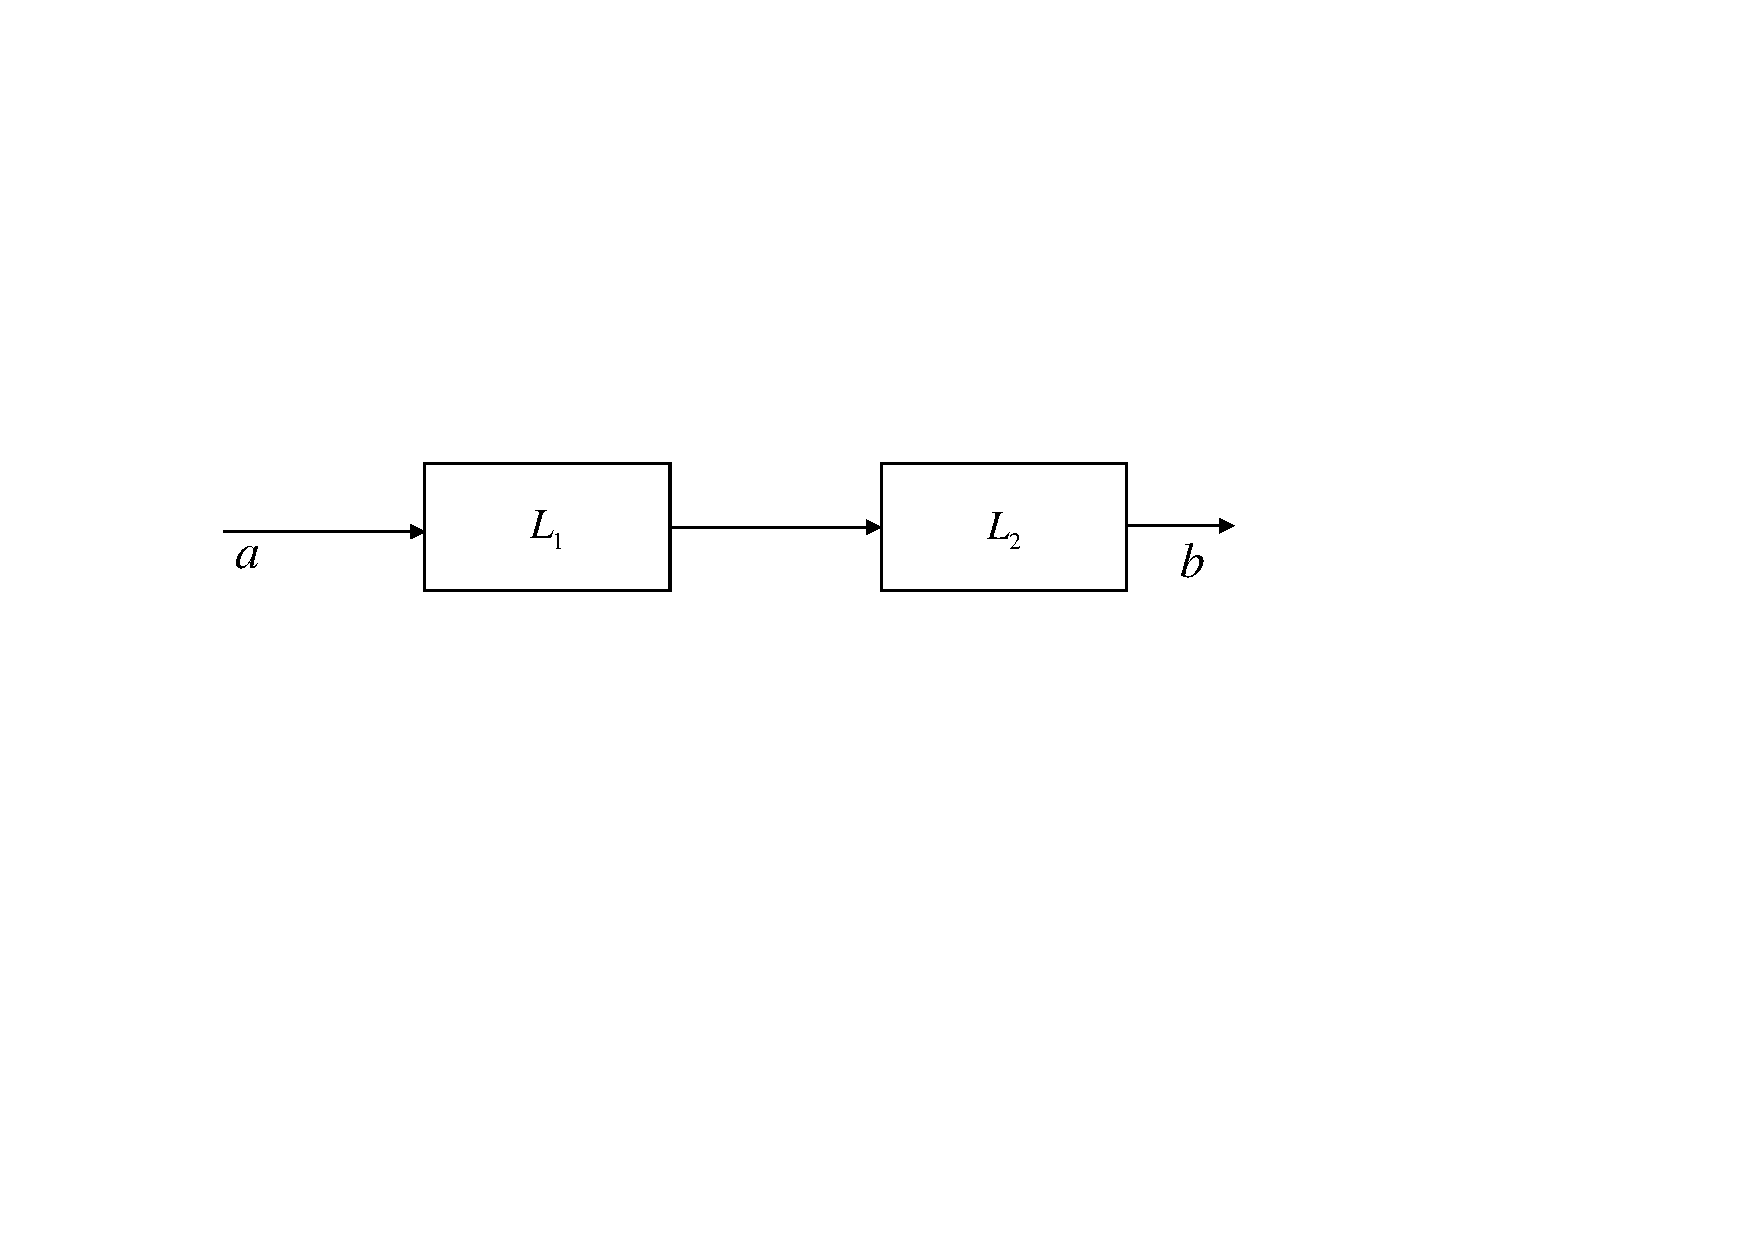
\includegraphics[width=0.4\textwidth]{3.pdf}
    \end{figure}
    \vspace{-0.5cm}
    \clearpage



    \item 甲乙两人轮流掷一颗骰子,每轮掷一次,谁先掷得6点谁得胜,从甲开始掷,问甲、乙得胜的
    概率各为多少?
    \clearpage



    \item 将一颗骰子掷两次,考虑事件: $A=\mbox{“第一次掷得点数2或5”}$.$B=\mbox{“两次点数之和至少为7”}$,
    求$P(A),P(B)$,并问事件$A,B$是否相互独立.
    \clearpage


    \item $A,B$两人轮流射击,每次每人射击一枪,射击的次序为$A,B,A,B,A,\cdots$,射击直至击
    中两枪为止.设每人击中的概率均为$p$,且各次击中与否相互独立.求击中的两枪是由同一人
    射击的概率.(提示:分别考虑两枪是由$A$击中的与两枪是由$B$击中的两种情况,若两枪是由
    $A$击中的,则射击必然在奇数次结束.又当$|x|<1$时,$1+2x+3x^2+\cdots=1/(1-x)^2$.)
    \clearpage



    \item 有3个独立工作的元件1,元件2,元件3,它们的可靠性分别为$p_1,p_2,p_3$.设由它们组
    成一个“3个元件取2个元件的表决系统”,记为$2/3[G]$. 这一系统的运行方式是当且仅当3个元件中至少有2个正
    常工作时这一系统正常工作.求这一$2/3[G]$系统的可靠性.
    \clearpage


    \item 在如图所示的桥式结构的电路中,第$i$个继电器触点闭合的概率为$p_i,i=1,2,3,4,5$.各继电器工作相互
    独立,求:
    \begin{enumerate}
        \item 以继电器触点1是否闭合为条件,求$A$到$B$之间为通路的概率.
        \item 已知$A$到$B$为通路的条件下,继电器触点3是闭合的概率.
    \end{enumerate}
    \begin{figure}[H]
        \flushright 
        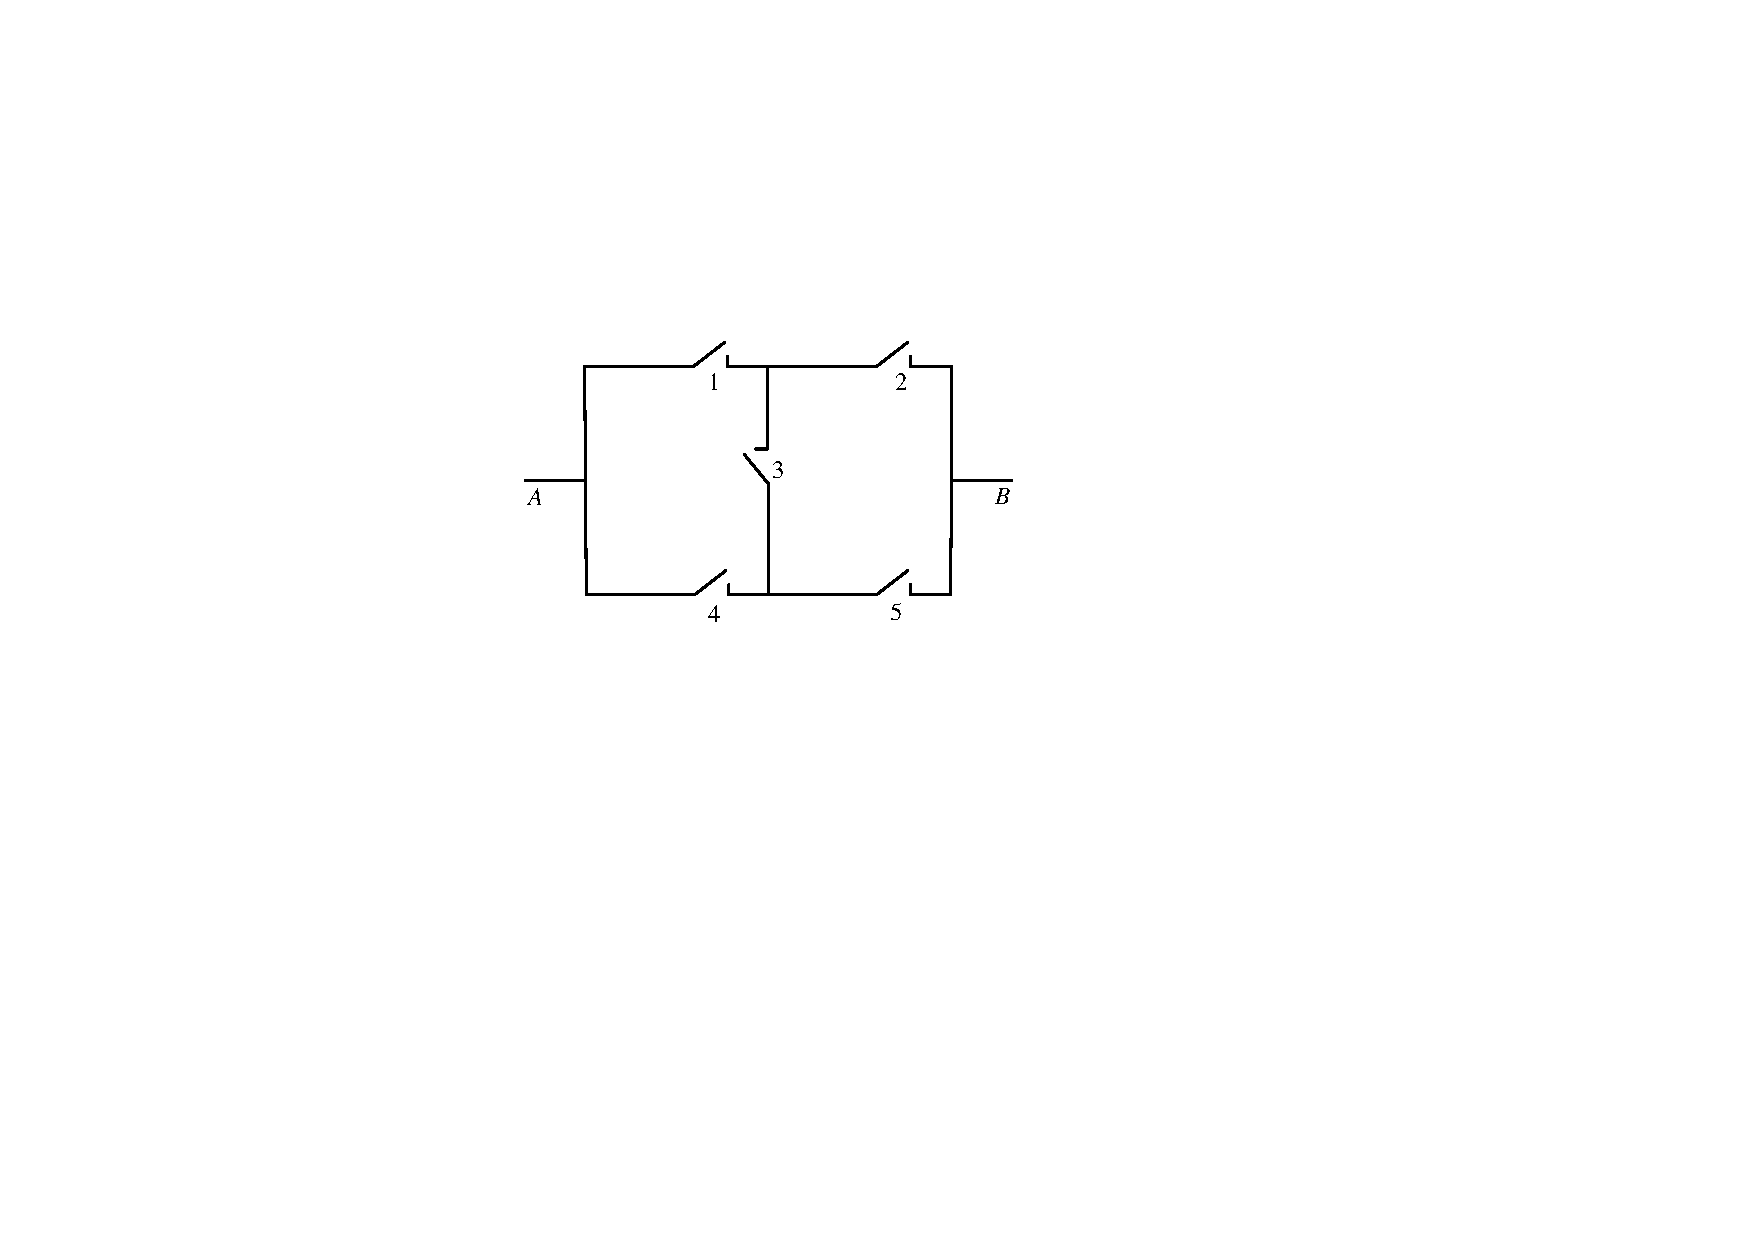
\includegraphics[width=0.25\textwidth]{8.pdf}
    \end{figure}
    \vspace{-0.5cm}
    \clearpage



    \item 进行非学历考试,规定考甲、乙两门课程,每门课程考试第一次未通过都只允许考第二
    次.考生仅在课程甲通过后才能考课程乙.如两门课程都通过可获得一张资格证书.设某考生
    通过课程甲的各次考试的概率为$p_1$,通过课程乙的各次考试的概率为$p_2$,设各次考试的结果
    相互独立.又设考生参加考试直至获得资格证书或者不准予再考为止.以$X$表示考生总共需
    考试的次数.求$X$的分布律.
    \clearpage


    \item \begin{enumerate}
        \item 5只电池,其中有2只是次品,每次取一只测试,直到将2只次品都找到.设第
        2只次品在第$X(X=2,3,4,5)$次找到,求$X$的分布律(注:在实际上第5次检测可无需进
        行).
        \item 5只电池,其中2只是次品,每次取一只,直到找出2只次品或3只正品为止.写出需
        要测试的次数的分布律.
    \end{enumerate}
    \clearpage


    \item 向某一目标发射炮弹,设炮弹弹着点离目标的距离为$R$(单位:10$\, $m),$R$服从瑞利分
    布,其概率密度为
    \vspace{-0.5cm}
    \begin{spacing}{2.0}
    $$f_R(r)=\left\{\begin{array}{ll}
        \dfrac{2r}{25}e^{-r^2/25},& r>0\\
        0, & r\leq 0
    \end{array}\right.$$
    \end{spacing}
    \vspace{-0.5cm}
    若弹着点离目标不超过5个单位时,目标被摧毁.
    \begin{enumerate}
        \item 求发射一枚炮弹能摧毁目标的概率.
        \item 为使至少有一枚炮弹能摧毁目标的概率不小于0.94,问最少需要独立发射多少枚
        炮弹.
    \end{enumerate}
    \clearpage
    



    \item 设一枚深水炸弹击沉一潜水艇的概率为$1/3$,击伤的概率为$1/2$ ,击不中的概率为
    $1/6$.并设击伤两次也会导致潜水艇下沉.求施放4枚深水炸弹能击沉潜水艇的概率.(提示:
    先求击不沉的概率.)
    \clearpage


    \item 一盒中装有4只白球,8只黑球,从中取3只球,每次一只,作不放回抽样.
    \begin{enumerate}
        \item 求第1次和第3次都取到白球的概率(提示:考虑第二次的抽取.)
        \item 求在第1次取到白球的条件下,前3次都取到白球的概率.
    \end{enumerate}
    \clearpage



    \item 设元件的寿命$T$(以小时计)服从指数分布,分布函数为
    $$F(t)=\left\{\begin{array}{ll}
        1-e^{-0.03t}, & t>0\\
        0, & t\leq 0
    \end{array}\right.$$
    \begin{enumerate}
        \item 已知元件至少工作了30小时,求它能再至少工作20小时的概率.
        \item 由3个独立工作的此种元件组成一个$2/3[G]$系统(参见第7题).求这一系统的寿
        命$X>20$的概率.
    \end{enumerate}
    \clearpage


    \item \begin{enumerate}
        \item 已知随机变量$X$的概率密度为$f_X(x)=\dfrac{1}{2}e^{-|x|},-\infty< x<\infty$,求$X$的分布函数.
        \item 已知随机变量$X$的分布函数为$F_X(x)$,另有随机变量
        $$Y=\left\{\begin{array}{ll}
            1, & X>0\\
            -1, & X\leq 0
        \end{array}\right.$$
    \end{enumerate}
    试求$Y$的分布律和分布函数.
    \clearpage



    \item \begin{enumerate}
        \item 设随机变量$X$服从泊松分布,其分布律为
        $$P\{X=k\}=\frac{\lambda^ke^{-\lambda}}{k!},\quad k=0,1,2,\cdots,$$
        间当$k$取何值时$P\{X=k\}$为最大.
        \item 设随机变量$X$服从二项分布,其分布律为
        $$P\{X=k\}=\binom{n}{k}p^k(1-p)^{n-k},\quad k=0,1,2,\cdots,n$$
        问当$k$取何值时$P\{X=k\}$为最大.
    \end{enumerate}
    \clearpage

    
    \item 若离散型随机变量$X$具有分布律
    \renewcommand{\arraystretch}{1.8}
    \begin{table}[H]\centering
        \begin{tabular}{c|cccc}

        $X$   & 1 & 2   & $\cdots$ & $n$   \\ \hline
        $p_k$ & $\displaystyle{\frac{1}{n}}$  & $\displaystyle{\frac{1}{n}}$ & $\cdots$ & $\displaystyle{\frac{1}{n}}$
        \end{tabular}
    \end{table}
        \vspace{-0.5cm}
        称$X$服从取值为$1,2,\cdots,n$的离散型均匀分布.对于任意非负实数$x$,记$[x]$为不超过$x$的最
        大整数.设$U\sim U(0,1)$,证明$X= [nU]+1$服从取值为$1,2,\cdots,n$的离散型均匀分布.
    \renewcommand{\arraystretch}{1}
    \clearpage



    \item 设随机变量$X\sim U(-1,2)$,求$Y=|X|$的概率密度.
    \clearpage


    \item 设随机变量$X$的概率密度

    \vspace{-0.5cm}
    \begin{spacing}{2}
    $$f_R(r)=\left\{\begin{array}{ll}
        0, & x<0\\
        \dfrac{1}{2}, & 0\leq x <1\\
        \dfrac{1}{2x^2}, & 1\leq x <\infty
    \end{array}\right.$$
    \end{spacing}
    求$Y=\dfrac{1}{X}$的概率密度.
    \clearpage


    \item 设随机变量$X$服从以均值为$1/\lambda$的指数分布.验证随机变量$Y=[X]$服从以参数为
    $1-e^{-\lambda}$的几何分布.这一事实表明连续型随机变量的函数可以是离散型随机变量.
    \clearpage




    \item 投掷一枚硬币直至正面出现为止,引入随机变量
    \begin{equation}
        \begin{split}
            &X=\mbox{投掷总次数}\\
            &Y=\left\{\begin{array}{ll}
                1, & \mbox{若首次投掷得到正面},\\
                0, & \mbox{若首次投掷得到反面}.
            \end{array}\right.
        \end{split}
        \nonumber
    \end{equation}
    \begin{enumerate}
        \item 求$X$和$Y$的联合分布律及边缘分布律.
        \item 求条件概率$P\{X=1|Y=1\},P\{Y=2|X=1\}$.
    \end{enumerate}
    \clearpage


    
    \item 设随机变量$X\sim \pi(\lambda)$,随机变量$Y=\max\{X,2\}$ .试求$X$和$Y$的联合分布律及边缘分
    布律.
    \clearpage



    \item 设$X,Y$是相互独立的泊松随机变量,参数分别为$\lambda_1,\lambda_2$,求给定$X+Y=n$的条件下$X$的条件分布.
    \clearpage




    \item 一教授将两篇论文分别交给两个打字员打印.以$X,Y$分别表示第一篇和第二篇论文
    的印刷错误.设$X\sim \pi(\lambda),Y\sim \pi(\mu)$,$X,Y$相互独立.
    \begin{enumerate}
        \item 求$X,Y$的联合分布律.
        \item 求两篇论文总共至多1个错误的概率.
    \end{enumerate}
    \clearpage





    \item 一等边三角形$\triangle ROT$(如图)的边长为1,在三
    角形内随机地取点$Q(X,Y)$ (意指随机点$(X,Y)$在三角形$ROT$内均匀分布).
    \begin{enumerate}
        \item 写出随机变量$(X,Y)$的概率密度.
        \item 求点$Q$到底边$OT$的距离的分布函数.
    \end{enumerate}
    \begin{figure}[H]
        \flushright 
        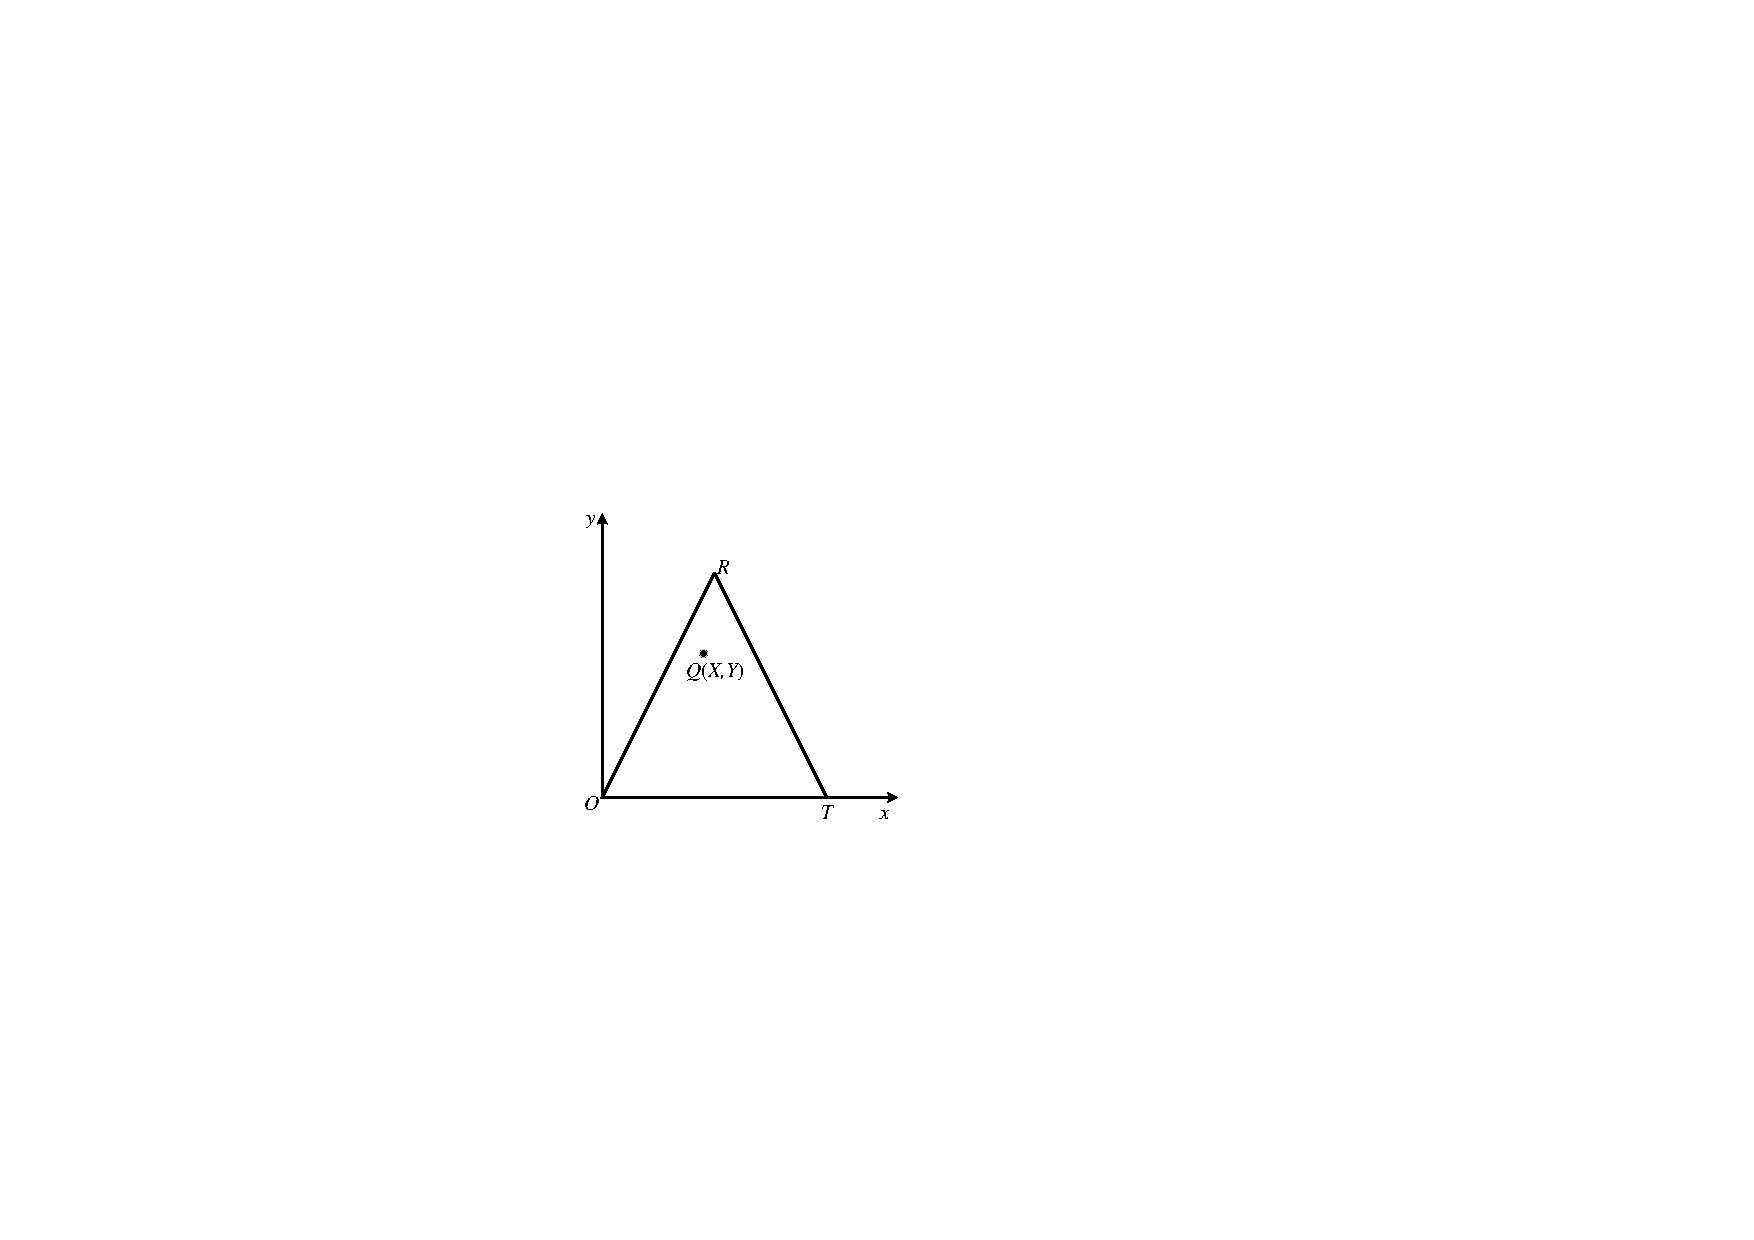
\includegraphics[width=0.2\textwidth]{25.pdf}
    \end{figure}
    \vspace{-0.5cm}
    \clearpage





    \item 设随机变量$(X,Y)$具有概率密度
    $$f(x,y)=\left\{\begin{array}{ll}
        xe^{-x(y+1)}, & x>0,y>0\\
        0, & \mbox{其他} 
    \end{array}\right.$$
    \begin{enumerate}
        \item 求边缘概率密度$f_X(x),f_Y(y)$.
        \item 求条件概率密度$f_{X|Y}(x|y),f_{Y|X}(y|x)$.
    \end{enumerate}
    \clearpage


    \item 设有随机变量$U$和$V$,它们都仅取$1,-1$两个值.已知
    \begin{equation}
        \begin{split}
            & P\{U=1\}=1/2,\\
            & P\{V=1|U=1\}=1/3=P\{V=-1|U=-1\}.
        \end{split}
        \nonumber
    \end{equation}
    \begin{enumerate}
        \item 求$U$和$V$的联合分布律.
        \item 求$x$的方程$x^2+Ux+V=0$至少有一个实根的概率.
        \item 求$x$的方程$x^2+(U+V)x+U+V=0$至少有一个实根的概率.
    \end{enumerate}
    \clearpage



    \item 某图书馆一天的读者人数$X\sim \pi(\lambda)$,任一读者借书的概率为$p$,各读者借书与否相互
    独立.记一天读者借书的人数为$Y$,求$X$和$Y$的联合分布律.
    \clearpage



    \item 设随机变量$X,Y$相互独立,且都服从均匀分布$U(0,1)$,求两变量之一至少为另一变
    量之值之两倍的概率.
    \clearpage


    \item 一家公司有一份保单招标,两家保险公司竞标.规定标书的保险费必须在20万元至
    22万元之间.若两份标书保险费相差2千或2千以上,招标公司将选择报价低者,否则就重
    新招标.设两家保险公司的报价是相互独立的,且都在20万至22万之间均匀分布.试求招标
    公司需重新招标的概率.
    \clearpage


    \item 设随机变量$X\sim N(0,\sigma_1^2),Y\sim N(0,\sigma_2^2)$且$X,Y$相互独立,求概率
    $$P\{0<\sigma_2 X -\sigma_1 Y<2\sigma_1\sigma_2\}$$
    \clearpage



    \item NBA篮球赛中有这样的规律,两支实力相当的球队比赛时,每节主队得分与客队得
    分之差为正态随机变量,均值为1.5,方差为6,并且假设四节的比分差是相互独立的.问:
    \begin{enumerate}
        \item 主队胜的概率有多大?
        \item 在前半场主队落后5分的情况下.主队得胜的概率有多大?
        \item 在第一节主队赢5分的情况下.主队得胜的概率有多大.
    \end{enumerate}
    \clearpage



    \item 产品的某种性能指标的测量值$X$是随机变量,设$X$的概率密度为
    $$f_X(x)=\left\{\begin{array}{ll}
        xe^{-\frac{1}{2}x^2}, & x>0\\
        0, & \mbox{其他}
    \end{array}\right.$$
    测量误差$Y\sim U(-\varepsilon ,\varepsilon),X,Y$ 相互独立.求$Z=X+Y$的概率密度$f_Z(z)$,并验证
    $$p\{Z>\varepsilon\}=\frac{1}{2\varepsilon}\int_0^{2\varepsilon} e^{-u^2/2}\mathrm{d}u$$
    \clearpage



    \item 在一化学过程中,产品中有份额$X$为杂质,而在杂质中有份额$Y$是有害的,而其余部
    分不影响产品的质量.设$X\sim U(0,0.1),Y\sim U(0,0.5)$,且$X$和$Y$相互独立.求产品中有害杂
    质份额$Z$的概率密度.
    \clearpage



    \item 设随机变量$(X,Y)$的概率密度为
    $$f(x,y)=\left\{\begin{array}{ll}
        e^{-y}, & 0<x<y\\
        0, & \mbox{其他}
    \end{array}\right.$$
    \begin{enumerate}
        \item 求$(X,Y)$的边缘概率密度.
        \item 问$X,Y$是否相互独立.
        \item 求$X+Y$的概率密度$f_{X+Y}(z)$.
        \item 求条件概率密度$f_{X|Y}(x|y)$.
        \item 求条件概率$P\{X>3|Y<5\}$.
        \item 求条件概率$P\{X>3|Y=5\}$.
    \end{enumerate}
    \clearpage


    \item 设某图书馆的读者借阅甲种图书的概率为$p$,借阅乙种图书的概率为$\alpha$,设每人借阅
    甲、乙图书的行动相互独立,读者之间的行动也相互独立.
    \begin{enumerate}
        \item 某天恰有$n$个读者,求借阅甲种图书的人数的数学期望.
        \item 某天恰有$n$个读者,求甲、乙两种图书中至少借阅一种的人数的数学期望.
    \end{enumerate}
    \clearpage



    \item 某种鸟在某时间区间$(0,t_0]$下蛋数为$1\sim 5$只,下$r$只蛋的概率与$r$成正比.一个收拾
    鸟蛋的人在时刻$t_0$去收集鸟蛋,但他仅当鸟窝中多于3只蛋时才从中取走一只蛋.在某处有
    这种鸟的鸟窝6个(每个鸟窝保存完好,各鸟窝中蛋的只数相互独立).
    \begin{enumerate}
        \item 写出一个鸟窝中鸟蛋只数$X$的分布律.
        \item 对于指定的一个鸟窝,求拾蛋人在该鸟窝中拾到一只蛋的概率.
        \item 求拾蛋人在6个鸟窝中拾到蛋的总数$Y$的分布律及数学期望.
        \item 求$P\{Y<4\},P\{Y>4\}$.
        \item 当一个拾蛋人在这6个鸟窝中拾过蛋后,紧接着又有一个拾蛋人到这些鸟窝中拾
        蛋,也仅当鸟窝中多于3只蛋时,拾取一只蛋,求第二个拾蛋人拾得蛋数$Z$的数学期望.
    \end{enumerate}
    \clearpage



    \item 设袋中有$r$只白球,$N-r$只黑球.在袋中取球$n(n\leq r)$次,每次任取一只作不放回抽
    样,以$Y$表示取到白球的个数,求$E(Y)$. (提示:引入随机变量:
    $$X_i=\left\{\begin{array}{ll}
        1, & \mbox{若第}i\mbox{次取到白球},\\
        0, & \mbox{若第}i\mbox{次取到黑球},
    \end{array}\right.\quad
    i=1,2,\cdots,n,$$
    则$Y=X_1+X_2+\cdots+X_n$).
    \clearpage


    \item 抛一颗骰子直到所有点数全部出现为止,求所需投掷次数$Y$的数学期望.(提示:令
    $X_1=1$,$X_2=$第一点得到后,等待第二个不同点所需的等待次数, $X_3=$第一二两点得到后,等
    待第三个不同点所需的等待次数,$X_4,X_5,X_6$类似,则$Y=X_1+X_2+\cdots+X_6$. 又几何分布
    $P\{X=k\}=(1-p)^{k-1}p,k=1,2,\cdots$的数学期望$E(X)=\frac{1}{p}$.)
    \clearpage


    \item 设随机变量$X,Y$相互独立.且$X,Y$分别服从以$1/\alpha,1/\beta$为均值的指数分布.求
    $E(X^2+Ye^{-X})$.
    \clearpage




    \item 一酒吧间柜台前有6张凳子,服务员预测,若两个陌生人进来就座的话,他们之间至
    少相隔两张凳子.(提示:先列出两人之间至少隔两张凳子的不同情况.)
    \begin{enumerate}
        \item 若真有两个陌生人入内,他们随机地就座,问服务员预言为真的概率是多少?
        \item 设两位顾客是随机就座的.求顾客之间凳子数的数学期望.
    \end{enumerate}
    \clearpage



    \item 设随机变量$X_1,X_2,\cdots,X_{100}$相互独立,且都服从$U(0,1)$,又设$Y=X_1X_2 \cdots X_{100}$,
    求概率$P\{Y<10^{-40}\}$的近似值.
    \clearpage


    \item 来自某个城市的长途电话呼唤的持续时间$X$(以分计)是一个随机变量,它的分布函
    数是
    $$F(x)=\left\{\begin{array}{ll}
        1-\dfrac{1}{2}e^{-\frac{x}{3}}-\dfrac{1}{2}e^{-[\frac{x}{3}]}, & x\leq 0\\
        0, & x<0
    \end{array}\right.$$
    (其中$[\dfrac{x}{3}]$是不大于$\dfrac{x}{3}$的最大整数).
    \begin{enumerate}
        \item 画出$F(x)$的图形.
        \item 说明$X$是什么类型的随机变量.
        \item 求$P\{X=4\},P\{X=3\},P\{X<4\},P\{X>6\}$. (提示:$P\{X=a\}=F(a)-F(a-0)$.)
    \end{enumerate}
    \clearpage



    \item 一汽车保险公司分析一组(250人)签约的客户中的赔付情况.据历史数据分析,在未
    来的一周中一组客户中至少提出一项索赔的客户数$X$占$10\%$.写出$X$的分布,并求$X>250\times 0.12$
   (即$X>30$) 的概率.设各客户是否提出索赔相互独立.
   \clearpage


   \item 在区间$(0,1)$随机地取一点$X$. 定义$Y=\min \{X,0.75\}$.
   \begin{enumerate}
       \item 求随机变量$Y$的值域.
       \item 求$Y$的分布函数,并画出它的图形.
       \item 说明$Y$不是连续型的随机变量,$Y$也不是离散型的随机变量.
   \end{enumerate}

    

    

  

\end{enumerate}
\end{document}